\let\negmedspace\undefined
\let\negthickspace\undefined
\documentclass[journal]{IEEEtran}
\usepackage[a5paper, margin=10mm, onecolumn]{geometry}
%\usepackage{lmodern} % Ensure lmodern is loaded for pdflatex
\usepackage{tfrupee} % Include tfrupee package

\setlength{\headheight}{1cm} % Set the height of the header box
\setlength{\headsep}{0mm}     % Set the distance between the header box and the top of the text

\usepackage{gvv-book}
\usepackage{gvv}
\usepackage{cite}
\usepackage{amsmath,amssymb,amsfonts,amsthm}
\usepackage{algorithmic}
\usepackage{graphicx}
\usepackage{textcomp}
\usepackage{xcolor}
\usepackage{txfonts}
\usepackage{listings}
\usepackage{enumitem}
\usepackage{mathtools}
\usepackage{gensymb}
\usepackage{comment}
\usepackage[breaklinks=true]{hyperref}
\usepackage{tkz-euclide} 
\usepackage{listings}
% \usepackage{gvv}                                        
\def\inputGnumericTable{}                                 
\usepackage[latin1]{inputenc}                                
\usepackage{color}                                            
\usepackage{array}                                            
\usepackage{longtable}                                       
\usepackage{calc}                                             
\usepackage{multirow}                                         
\usepackage{hhline}                                           
\usepackage{ifthen}                                           
\usepackage{lscape}
\usepackage{circuitikz}
\tikzstyle{block} = [rectangle, draw, fill=blue!20, 
    text width=4em, text centered, rounded corners, minimum height=3em]
\tikzstyle{sum} = [draw, fill=blue!10, circle, minimum size=1cm, node distance=1.5cm]
\tikzstyle{input} = [coordinate]
\tikzstyle{output} = [coordinate]


\begin{document}

\bibliographystyle{IEEEtran}
\vspace{3cm}

\title{2.7.21}
\author{EE25BTECH11009-Anshu kumar ram}
 \maketitle
% \newpage
% \bigskip
{\let\newpage\relax\maketitle}

\renewcommand{\thefigure}{\theenumi}
\renewcommand{\thetable}{\theenumi}
\setlength{\intextsep}{10pt} % Space between text and floats


\numberwithin{equation}{enumi}
\numberwithin{figure}{enumi}
\renewcommand{\thetable}{\theenumi}

\textbf{Question}:\\
Find the values of $k$ so that the area of the triangle with vertices 
$A(1,-1),\; B(-4,2k),\; C(-k,-5)$ is $24$ sq. units.

\solution \\

The given vertices are
\begin{tabular}{|c|c|}
\hline
\textbf{Name} & \textbf{Value} \\ \hline
$\vec{A}$ & $\myvec{2 & 1 \\0 & 3}$ \\ \hline
\end{tabular}

\begin{align}
    \vec{u} &= \vec{B}-\vec{A} = \myvec{-5 \\ 2k+1}, \\
    \vec{v} &= \vec{C}-\vec{A} = \myvec{-k-1 \\ -4}.
\end{align}

The area of $\triangle ABC$ is
\begin{align}
    \Delta &= \frac{1}{2}\norm{\vec{u}\times \vec{v}}.
\end{align}

Using the identity
\begin{align}
    \norm{\vec{u}\times\vec{v}}^2 
    &= \norm{\vec{u}}^2\norm{\vec{v}}^2 - (\vec{u}^\top\vec{v})^2
\end{align}

Hence,
\begin{align}
    \norm{\vec{u}\times\vec{v}}^2 
    &= (2k^2+3k+21)^2
\end{align}
\begin{align}
    \implies \norm{\vec{u}\times\vec{v}} &= \abs{2k^2+3k+21}.
\end{align}

So,
\begin{align}
    \Delta &= \frac{1}{2}\abs{2k^2+3k+21}.
\end{align}

Given $\Delta=24$,
\begin{align}
    \abs{2k^2+3k+21} &= 48
\end{align}

\textbf{Case 1:}
\begin{align}
    2k^2+3k+21 = 48 \\
    \implies 2k^2+3k-27=0
\end{align}
\begin{align}
    k &= \frac{-3\pm 15}{4} = \{3,\;-\tfrac{9}{2}\}
\end{align}

\textbf{Case 2:}
\begin{align}
    2k^2+3k+21 = -48 \\
    \implies 2k^2+3k+69=0
\end{align}
This has no real roots.

\begin{align}
    \therefore k \in \left\{3,\; -\tfrac{9}{2}\right\}
\end{align}

\begin{table}[h!]
    \centering
    \begin{tabular}{|c|c|c|}
        \hline
        Point & For $k=3$ & For $k=-\tfrac{9}{2}$ \\
        \hline
        $A$ & $\myvec{1\\-1}$ & $\myvec{1\\-1}$ \\
$B$ & $\myvec{-4\\6}$ & $\myvec{-4\\-9}$ \\
$C$ & $\myvec{-3\\-5}$ & $\myvec{\tfrac{9}{2}\\-5}$ \\
        \hline
    \end{tabular}
    \caption{Vertices of $\triangle ABC$ after substituting $k$ values}
    \label{tab:triangle_values}
\end{table}

  

\begin{figure}[h!]
    \centering
    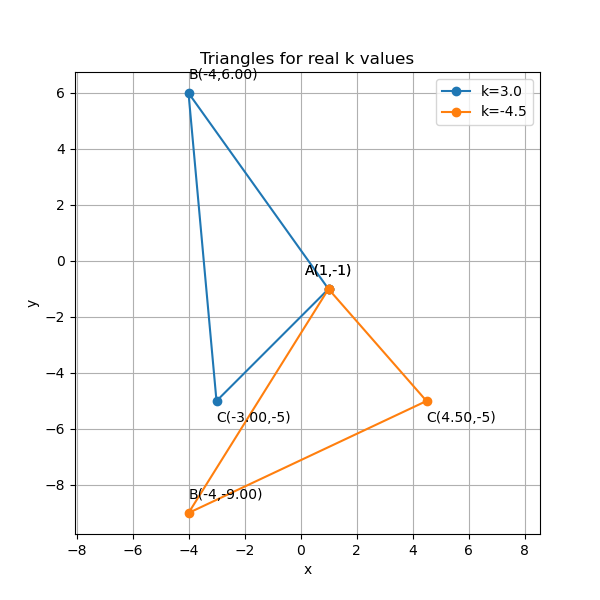
\includegraphics[width=\columnwidth, keepaspectratio]{figs/triangle_area.png}
    \label{fig:triangle_area}
\end{figure}

\end{document}
